\documentclass[a4j,10pt,dvipdfmx]{jarticle}
\usepackage{url}
\usepackage[version=3]{mhchem}
\usepackage{siunitx}
\usepackage[dvipdfmx]{graphicx}
\usepackage{pdfpages}
\usepackage{here}
\usepackage{tabularx}
\author{学籍番号2120029, 氏名 政野玄空}
\date{2023年6月22日}
\begin{document}
\section{実験目的}
反転増幅回路と加算回路を作成し,演算増幅器とも呼ばれるオペアンプの特徴について理解し,オペアンプを用いた回路設計の一般的手法を学ぶ.
\section{原理}

\subsection{オペアンプについて}
オペアンプは,2つの入力の差分を増幅して出力できる集積回路で,アナログ回路で微分,積分,加算,減算,比較の演算ができるのが特徴である.複数のピンがあり,駆動するための電源の端子,非反転と反転の2つの入力端子,それの対になる出力端子がある.

実験で用いたTL074CNには4つのオペアンプがあり,電源電圧$V_{CC+}$,$V_{CC-}$を加え,各端子を利用できる.

オペアンプの出力電圧を$V_o$とすると,$V_o$は2つの入力端子の電位差に開放電圧利得($A$)をかけた値になり
\begin{eqnarray}
  \label{V_o}
  V_o = A(V_{+}-V_{-})
\end{eqnarray}
となる.

オペアンプは内部のモジュール回路の作用により,2つの入力端子の電位差が生じないようになっている.このことをバーチャルショートと呼ぶ.その特徴を利用して$V_{+}$,$V_{-}$に電位差が生じるような構造にして,差分$\Delta V$を利得係数$A_V$で増幅して信号を得る.
入力端子の片方は基準電圧入力端子,もう一方は帰還信号入力端子とするのが一般的で,負帰還をかけることにより増幅度を抑え安定させている.

\subsection{反転増幅回路}
反転増幅回路は反転入力端子$V_-$に抵抗$R_1$を介して信号を加え,出力$V_o$から$R_2$を介して負帰還を加える構成となる.反転入力端子に信号を加えるため,入力と出力の位相は反転する.

反転増幅回路を図に示す.
\begin{figure}[H]
  \begin{center}
  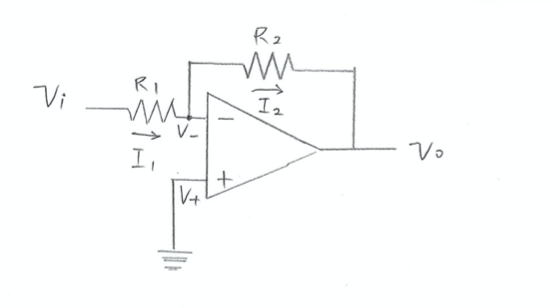
\includegraphics[height=7cm,width=10cm]{hanpuku.png}
  \caption{反転動作回路}
\end{center}
\end{figure}
バーチャルショートを保つことより,$V_-$と$V_+$は等しくなる.入力インピーダンスが高いため$R_1$を通った電流はすべて$R_2$に流れる.よって$R_1$に流れる電流と$R_2$に流れる電流は等しい.
よって
\begin{eqnarray}
  \label{icib}
\frac{{V_i}-{V_-}}{R_1} = \frac{{V_-}-{V_o}}{R_2} 
\end{eqnarray}
\begin{eqnarray}
  \label{Av}
A_V=\frac{V_o}{V_i} = -\frac{R_2}{R_1} 
\end{eqnarray}
となる.
\subsection{加算回路}
反転増幅回路と同様に$V_-$と$V_+$は等しい.

加算回路を図に示す.
\begin{figure}[H]
  \begin{center}
  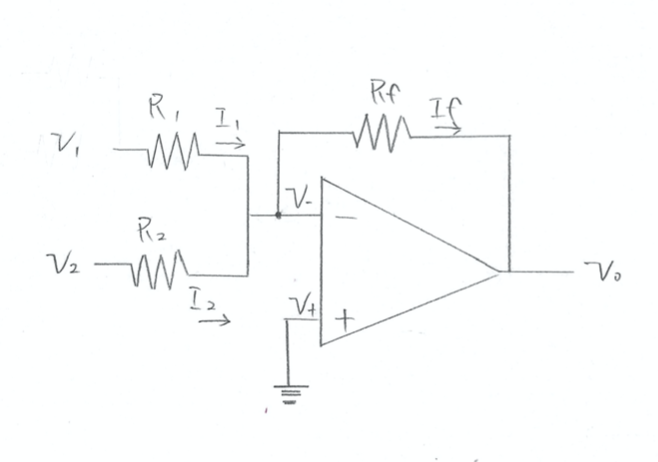
\includegraphics[height=7cm,width=10cm]{kasan.png}
  \caption{加算回路}
\end{center}
\end{figure}
加算回路は,反転増幅回路の入力を2つにしたものと考えることができるので,$R_1$と$R_2$の電流を一旦$R_{12}$とし,,$V_1$と$V_2$を$V_i$とおく.
1.と同様に入力インピーダンスが高いため$R_{12}$を通った電流はすべて$R_f$に流れる.よって$R_{12}$に流れる電流と$R_f$に流れる電流は等しい.
\begin{eqnarray}
  \label{vvvvvvvv}
\frac{{V_i}-{V_-}}{R_{12}} =  \frac{{V_-}-{V_o}}{R_f} 
\end{eqnarray}
$R_{12}$を$R_1$と$R_2$に戻すと
  \begin{eqnarray}
    \label{vvvvvvvvv}
  \frac{{V_1}-{V_-}}{R_1} + \frac{{V_2}-{V_-}}{R_2} =  \frac{{V_-}-{V_o}}{R_f} 
  \end{eqnarray}
  $V_+$が接地してあることより
  \begin{eqnarray}
    \label{voi}
  V_+ = V_- = 0
  \end{eqnarray}
(\ref{vvvvvvvvv})に(\ref{voi})を代入して整理すると
\begin{eqnarray}
  \label{voqi}
V_o = -(\frac{R_f}{R_1}V_1+\frac{R_f}{R_2}V_2)
\end{eqnarray}
となる.
\section{実験方法}
\subsection{反転増幅回路の測定}
\begin{enumerate}
  \item $R_1$10$k\Omega$,$R_2$の抵抗100$k\Omega$を準備しディジタルマルチネーターで実測する.
  \item シュミレーションソースを用いて測った値を入力し,シュミレーターの$V_i$と$V_o$を測定点とする.
  \item 波形を確認する.同様に非反転増幅回路も確認する.
  \item 測定した抵抗を用いて反転増幅回路を実装する.
  \item オペアンプに電源電圧を加える.このとき正負をよく確認する.GND基準電位として連結された直流固定電源2台の中点電位を配線する.
  \item 交流信号源としてファンクションジェネレータの赤の信号線を抵抗$R_1$手前の$V_i$の位置に接続する.
  \item オシロスコープをCH1を$V_i$,CH2を$V_o$に接続する.両方ともGNDはファンクションジェネレータのGNDかつ直流固定電源のGNDと同電位の位置へ接続する.設定は10×,AC結合にする.
  \item バッファアンプの電源を入れて,ファンクションジェネレータと直流固定電源の出力をONにする.
  \item ファンクションジェネレータの出力周波数を1kHz,Vppを0から4.8Vppまで0.4感覚で$V_i$,$V_o$のVpp値を測定する.途中でオシロスコープ上の波形も確認する.
  \item 測定結果から入出力電圧特性グラフを作成する
\end{enumerate}
\subsection{加算回路の測定}

\begin{enumerate}
  \item C=1000pFのキャパシタンスをLCRメーターで測定する.
  \item $R_1$,$R_2$,$R_3$,$R_f$となる10$k\Omega$の抵抗をとり,.(\ref{kasanzu})の通り加算回路の実装をする.$v_1$,$v_2$の前段はボルテージフォロア回路と呼ばれ,その前段のRC位相回路の特性をそのままに,キャパシタ端子電圧を出力できる.
  \item 直流固定電源をオペアンプの電源電圧,GND端子につながるように配線する.
  \item 交流信号源としてファンクションジェネレータの赤の信号線を$v_1$に接続する.ファンクションジェネレータの黒のGNDを直流固定電源の中点のGND線と同様の場所に接続する.
  \item ファンクションジェネレータの出力設定を16kHz,8Vppに設定する.
  \item オシロスコープのCH1を$v_1$,CH2を最初は$v_2$,その次に$v_o$に繋ぎ変える.
  \item オシロスコープのカーソルを項目:時間,チャネル:CH1とし,$v_1$波形の立ち上がりが左端になるようにする.このときカーソル1の電圧は左端で0になる.カーソル2との$\Delta t$が10$\mu$sとなるように調整して電圧を読み取り$v_2$として記録する.波形画面を保存しておく.
  \item CH2を$v_o$に繋ぎ変える.チャネル:CH2のままカーソル2電圧を読み取り$v_o$として記録する..波形画面を保存しておく.
  \item $\Delta t$を適宜変更し何度か測定を繰り返す.
\end{enumerate}
\section{結果}

\subsection{反転増幅回路}
$R_1$,$R_2$の測定結果は,9.96$k\Omega$,100.0$k\Omega$であった.
電圧増幅度理論値はこの値より-10.03倍になる.


次にシュミレーションによる測定値の結果を示す.
まず反転増幅回路のシュミレーション結果の波形はこの様になった.
\begin{figure}[H]
  \begin{center}
  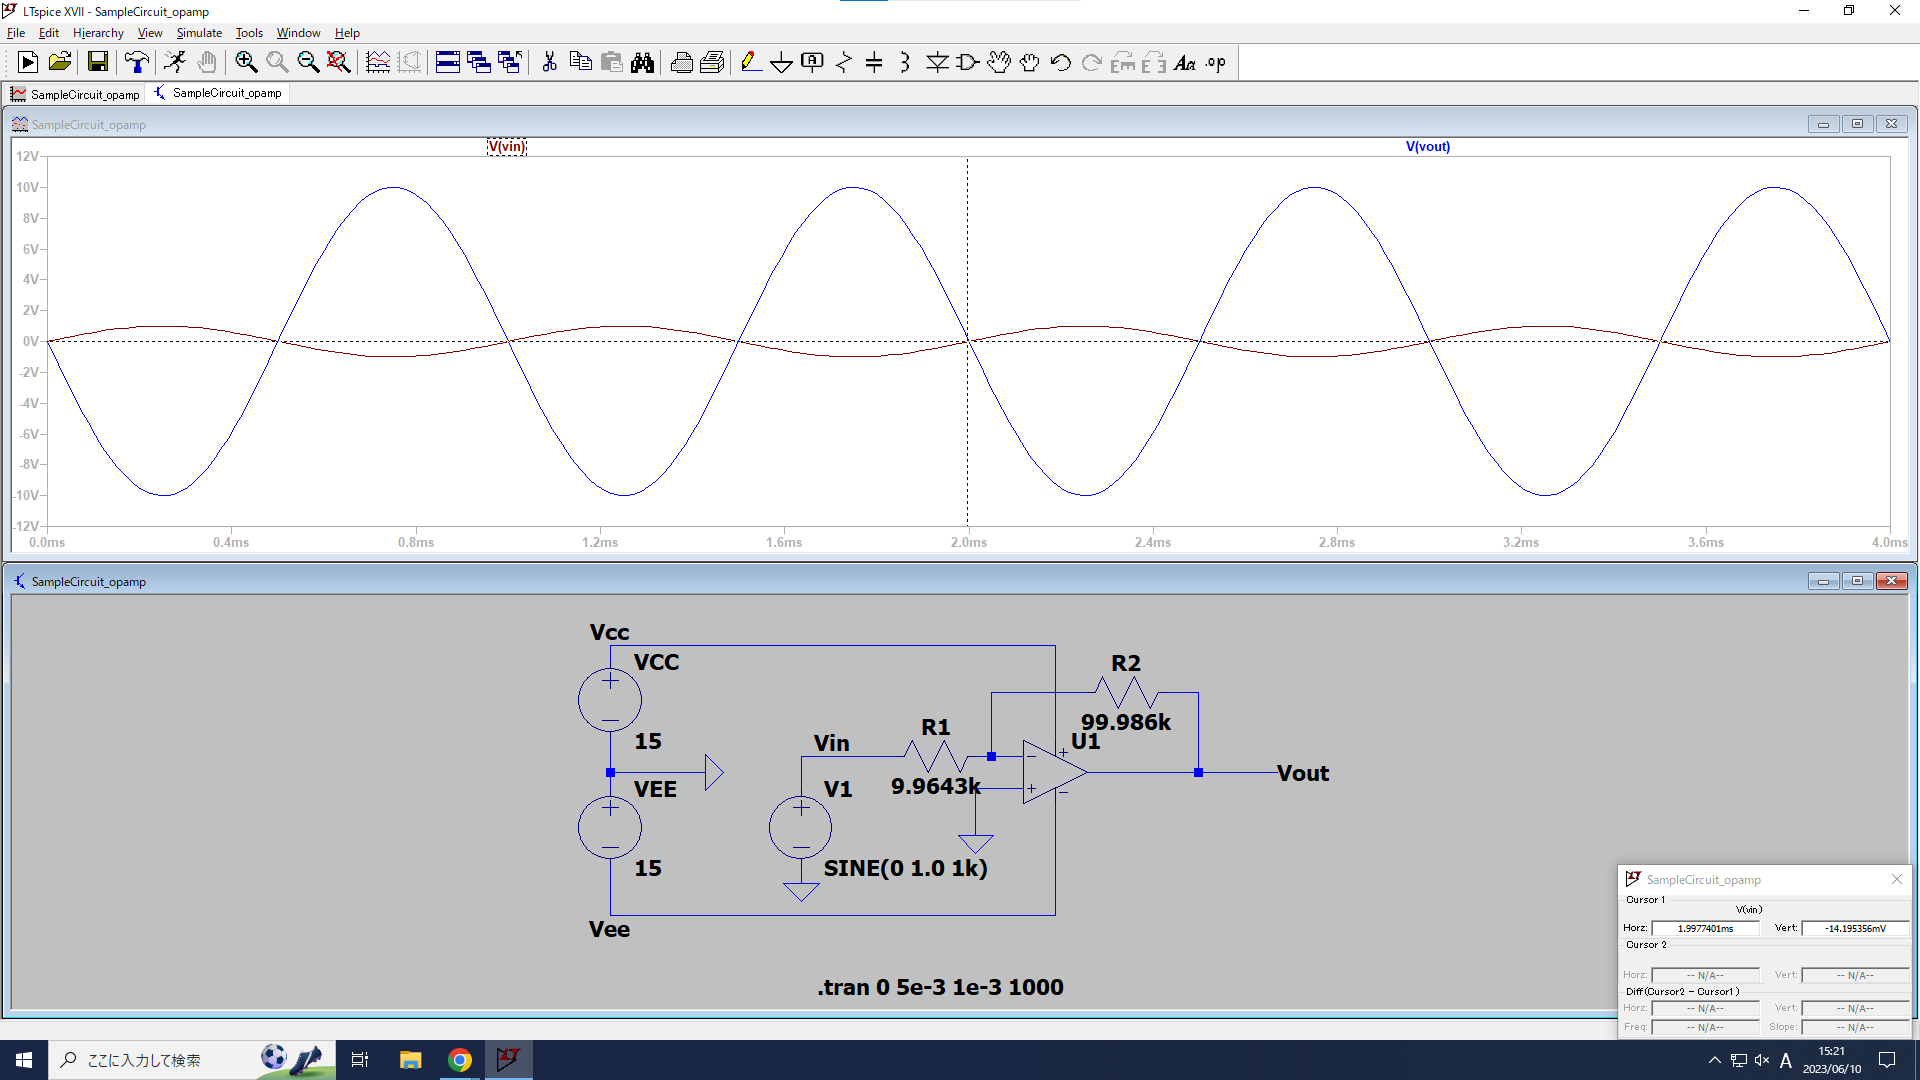
\includegraphics[height=7cm,width=10cm]{hantensimu.png}
  \caption{反転増幅回路のシュミレーション画面}
\end{center}
\end{figure}
次に非反転増幅回路のシュミレーション結果の波形はこの様になった.
\begin{figure}[H]
  \begin{center}
  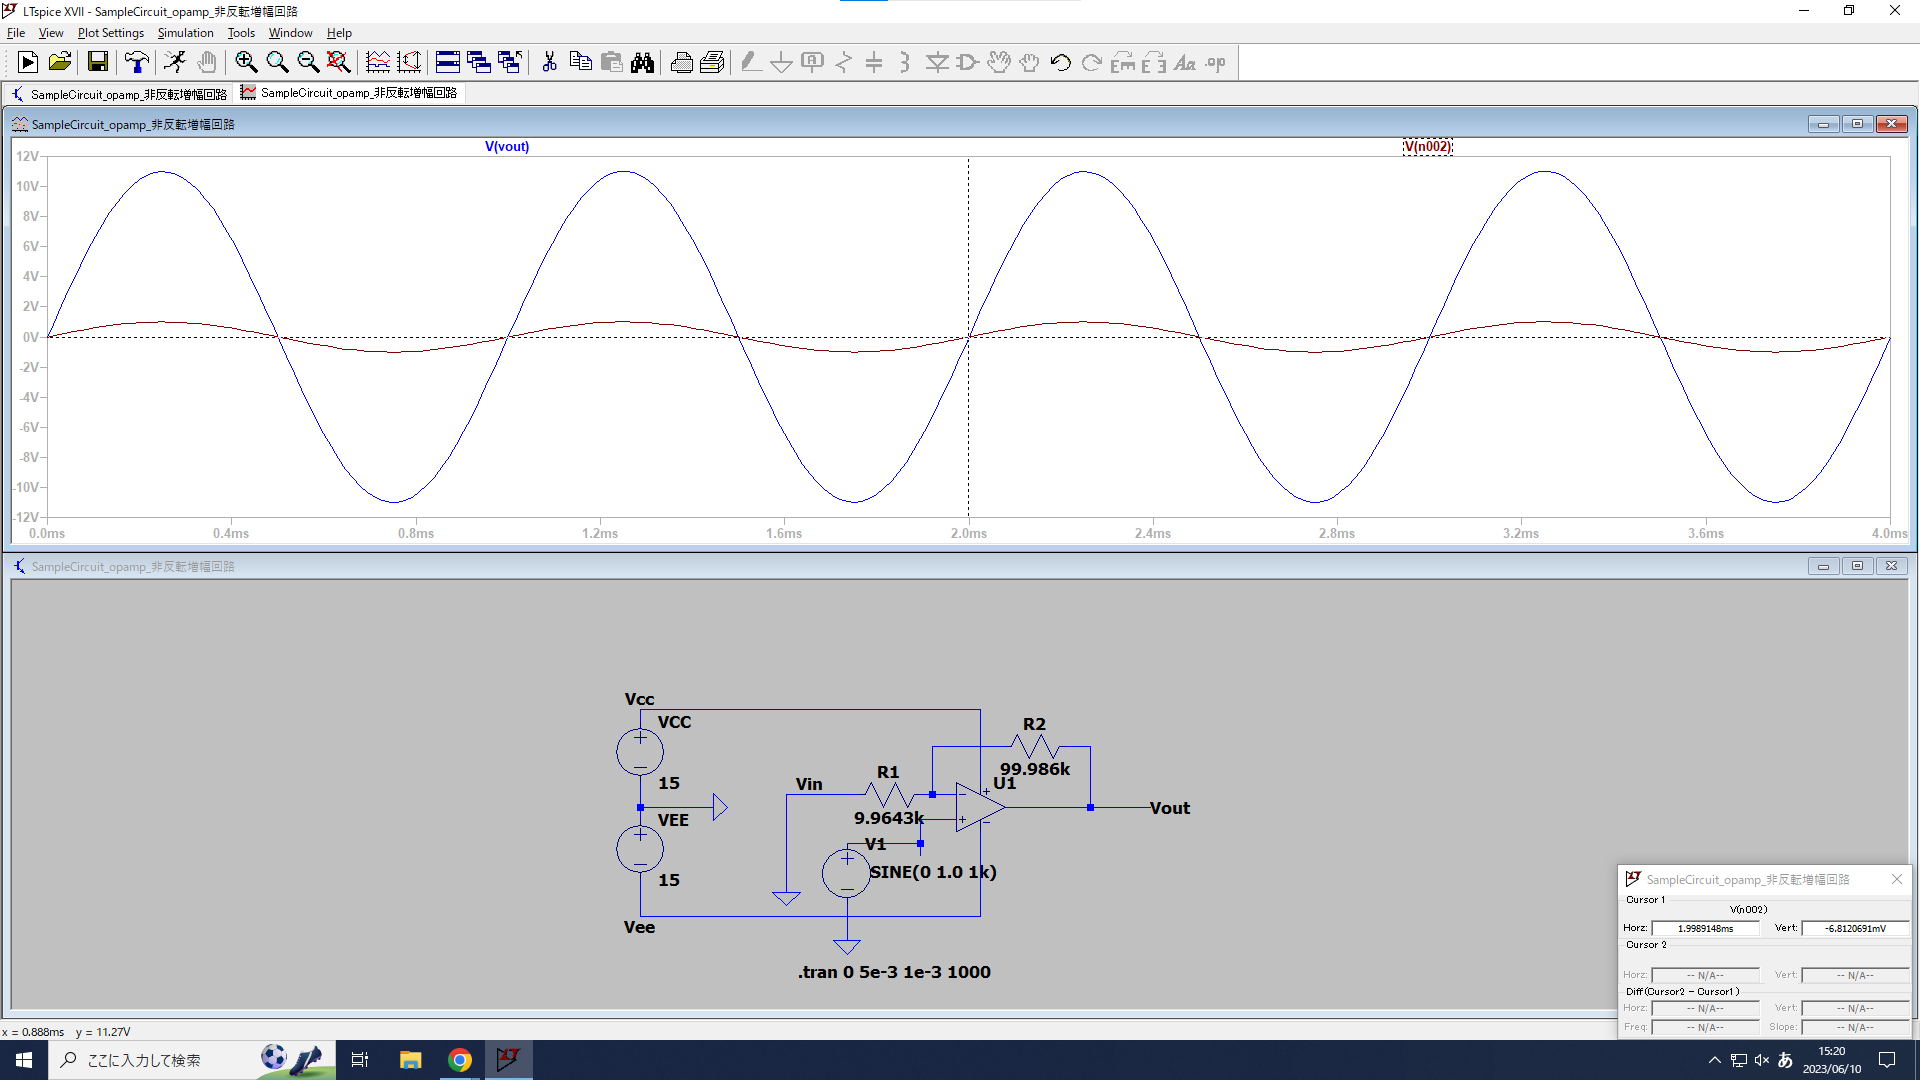
\includegraphics[height=7cm,width=10cm]{hihantensimu.png}
  \caption{非反転増幅回路のシュミレーション画面}
\end{center}
\end{figure}

次に反転増幅回路のシュミレーションの結果の数値を表にまとめたものを示す.
\begin{table}[H]
  \begin{center}
  \begin{tabular}{|l|l|l|l|}
  \hline
      XFG1の & \multicolumn{2}{|c|}{シミュレーションによる}  & 電圧増幅度 \\
      Vp設定値 & \multicolumn{2}{|c|}{カーソル測定値}  & \\ \hline
      vi[V] & vi[V] & vo[V] & -vo/vi \\ \hline
      0.0  & 0.0000 & 0.0000 &  \\ \hline
      0.2  & 0.3999 & 4.0029 & -10.01 \\ \hline
      0.4  & 0.8000 & 8.0058 & -10.01 \\ \hline
      0.6  & 1.2000 & 12.0085 & -10.01 \\ \hline
      0.8  & 1.6000 & 16.0127 & -10.01 \\ \hline
      1.0  & 1.9999 & 20.0160 & -10.01 \\ \hline
      1.2  & 2.4000 & 24.0224 & -10.01 \\ \hline
      1.4  & 2.7994 & 28.0290 & -10.013 \\ \hline
      1.6  & 3.2000 & 29.9968 & -9.374 \\ \hline
      1.8  & 3.5992 & 29.9968 & -8.334 \\ \hline
      2.0  & 3.9918 & 29.9968 & -7.515 \\ \hline
      2.2  & 4.3996 & 29.9968 & -6.818 \\ \hline
      2.4  & 4.7973 & 29.9968 & -6.253 \\ \hline
  \end{tabular}
  \caption{反転増幅回路のシュミレーション結果}
\end{center}
\end{table}
次にオシロスコープによる測定値を示す.
\begin{table}[H]
  \begin{center}
  \begin{tabular}{|l|l|l|l|}
  \hline
      FG & \multicolumn{2}{|c|}{オシロスコープによる}  & 電圧増幅度 \\
      出力値 & \multicolumn{2}{|c|}{Vpp測定値}  & \\ \hline
      Fgout [Vpp] & vi[V] & vo[V] & vo/vi [倍] \\ \hline
      0.0  & 0.14000 & 0.36000 & 2.57 \\ \hline
      0.4  & 0.520  & 4.30  & 8.27 \\ \hline
      0.8  & 0.920  & 8.50  & 9.24 \\ \hline
      1.2  & 1.35  & 12.5  & 9.26 \\ \hline
      1.6  & 1.77  & 17.3  & 9.77 \\ \hline
      2.0  & 2.15  & 21.3  & 9.91 \\ \hline
      2.4  & 2.57  & 25.3  & 9.84 \\ \hline
      2.8  & 2.97  & 29.0  & 9.76 \\ \hline
      3.2  & 3.38  & 29.3  & 8.67 \\ \hline
      3.6  & 3.80  & 29.5  & 7.76 \\ \hline
      4.0  & 4.22  & 29.5  & 6.99 \\ \hline
      4.4  & 4.62  & 29.5  & 6.39 \\ \hline
      4.8  & 5.11  & 29.5  & 5.77 \\ \hline
  \end{tabular}
  \caption{反転増幅回路の測定結果}
\end{center}
\end{table}
つぎに2.4Vppと4.0Vppのときのオシロスコープの画面を示す
\begin{figure}[H]
  \begin{center}
  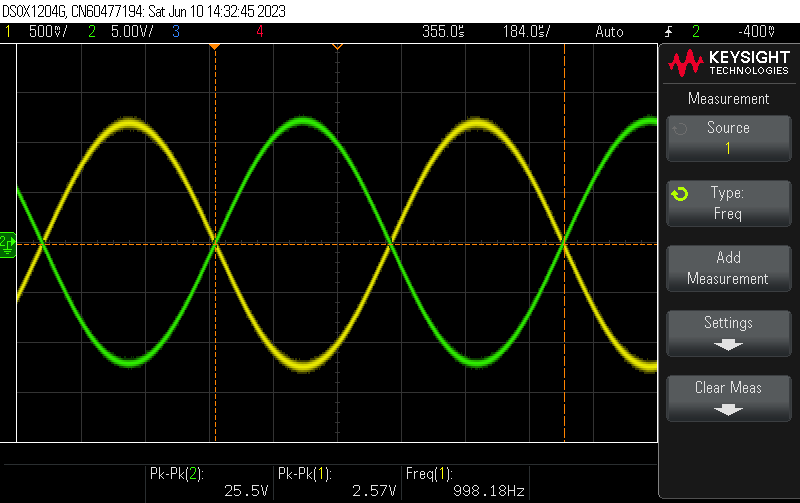
\includegraphics[height=7cm,width=10cm]{2.4Vpp.png}
  \caption{FG出力が2.4Vppのときの反転増幅回路のオシロスコープの波形}
\end{center}
\end{figure}
\begin{figure}[H]
  \begin{center}
  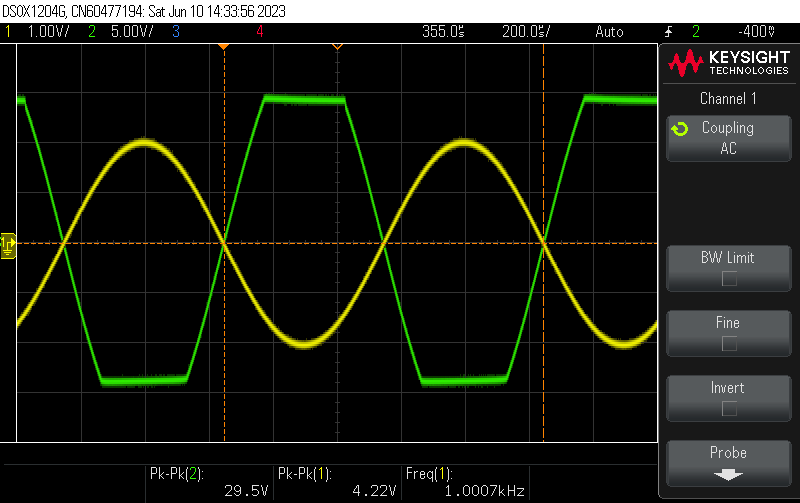
\includegraphics[height=7cm,width=10cm]{4Vpp.png}
  \caption{FG出力が4.0Vppのときの反転増幅回路のオシロスコープの波形}
\end{center}
\end{figure}
これらの結果をグラフにまとめるとこのようになる.
\begin{figure}[H]
  \begin{center}
  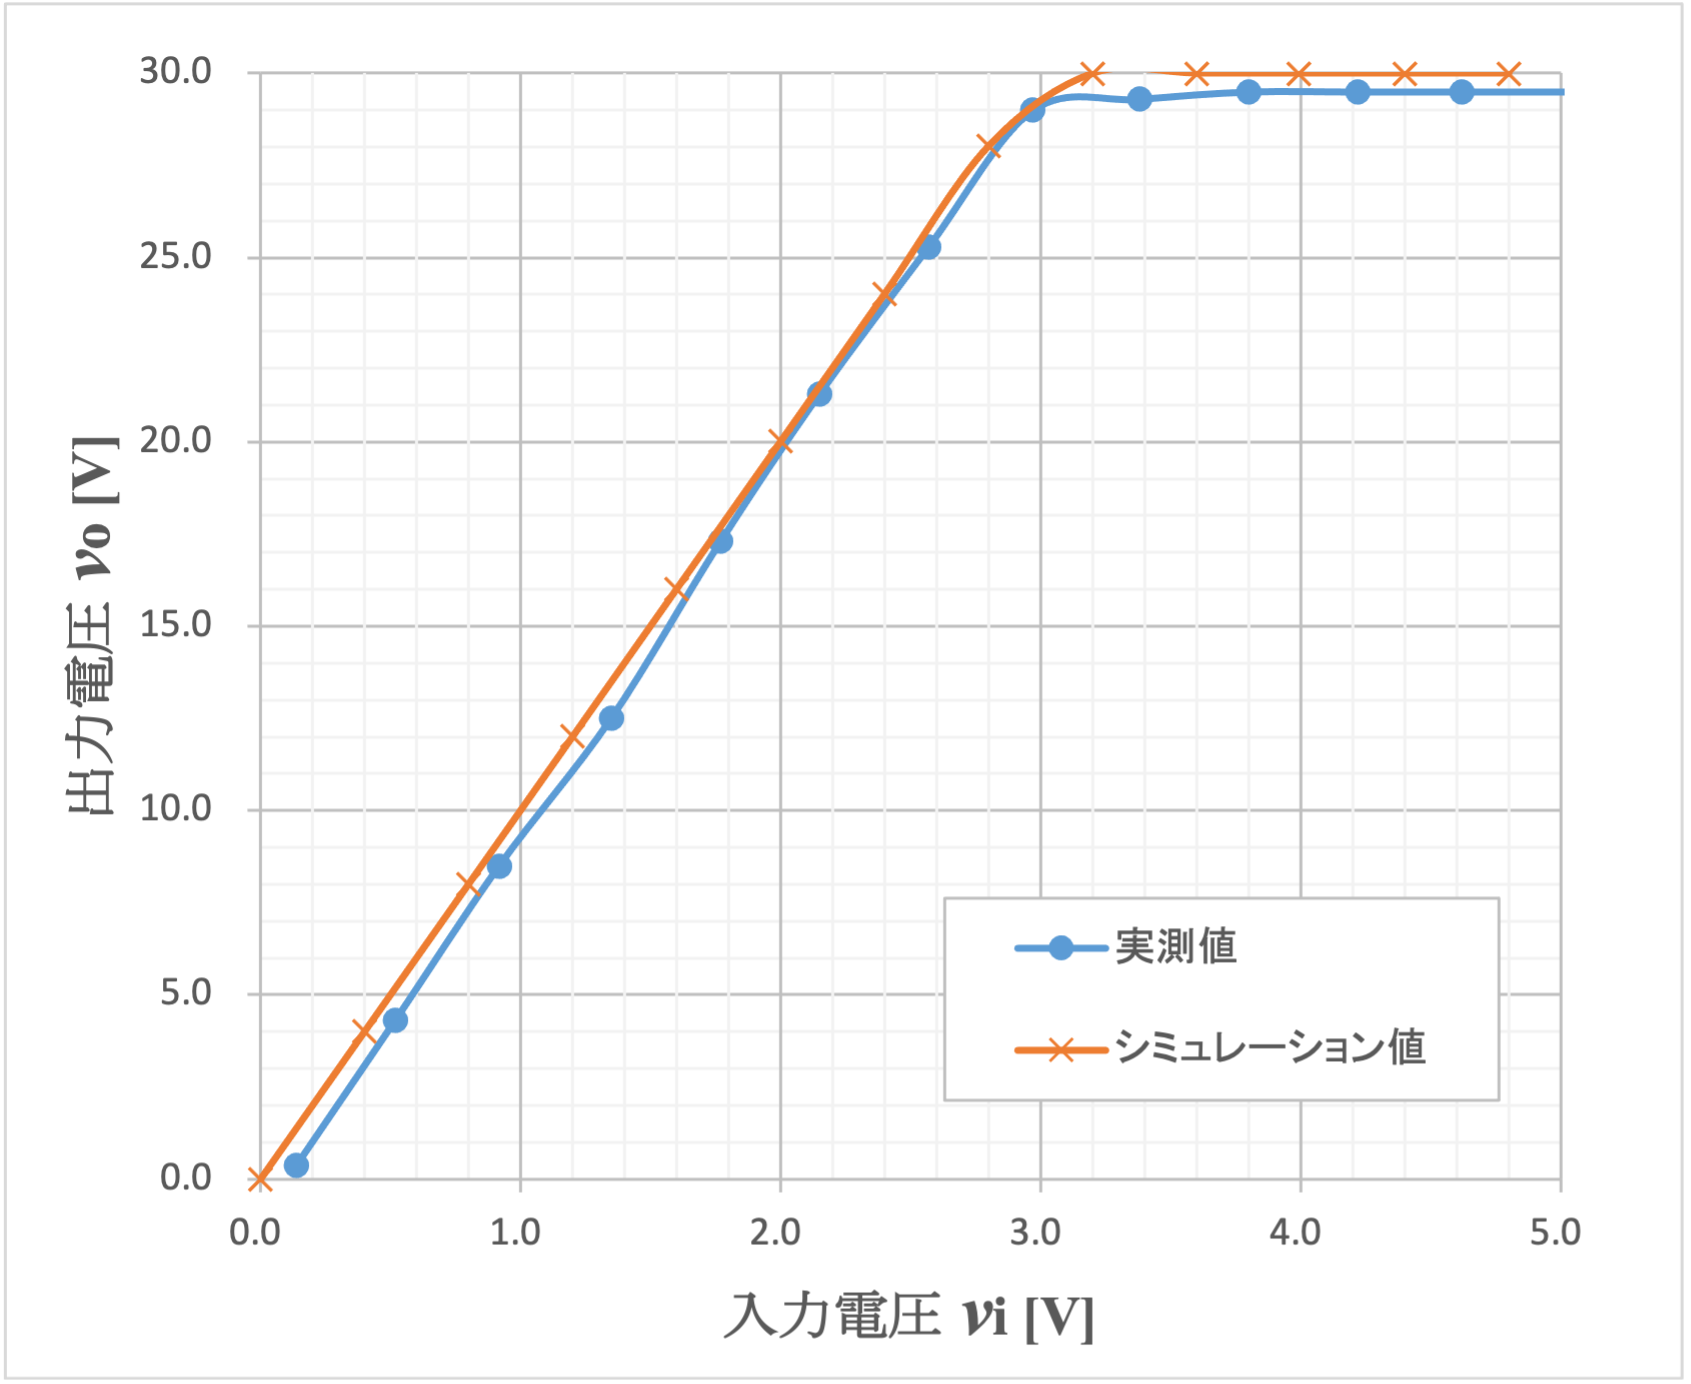
\includegraphics[height=7cm,width=10cm]{hantengurafu.png}
  \caption{反転増幅回路の電圧増幅特性}
\end{center}
\end{figure}

加えて非反転増幅回路の結果も同様に示す.

\begin{table}[H]
  \begin{center}
  \begin{tabular}{|l|l|l|l|}
  \hline
      XFG1の & \multicolumn{2}{|c|}{シミュレーションによる}  & 電圧増幅度 \\
      Vp設定値 & \multicolumn{2}{|c|}{カーソル測定値}  & \\ \hline
      vi[V] & vi[V] & vo[V] & -vo/vi \\ \hline
      0.0  & 0.0000 & 0.0000 &  \\ \hline
      0.2  & 0.3999 & 4.4027 & -11.01 \\ \hline
      0.4  & 0.7998 & 8.8054 & -11.01 \\ \hline
      0.6  & 1.2000 & 13.2098 & -11.01 \\ \hline
      0.8  & 1.5999 & 17.6100 & -11.01 \\ \hline
      1.0  & 1.9999 & 22.0100 & -11.01 \\ \hline
      1.2  & 2.3996 & 26.4122 & -11.01 \\ \hline
      1.4  & 2.8000 & 29.9970 & -10.713 \\ \hline
      1.6  & 3.2000 & 29.9972 & -9.374 \\ \hline
      1.8  & 3.5991 & 29.9972 & -8.335 \\ \hline
      2.0  & 3.9987 & 29.9972 & -7.502 \\ \hline
      2.2  & 4.3981 & 29.9972 & -6.820 \\ \hline
      2.4  & 4.7995 & 29.9972 & -6.250 \\ \hline
      2.8  & 2.97  & 29.0  & 9.76 \\ \hline
      3.2  & 3.38  & 29.3  & 8.67 \\ \hline
      3.6  & 3.80  & 29.5  & 7.76 \\ \hline
      4.0  & 4.22  & 29.5  & 6.99 \\ \hline
      4.4  & 4.62  & 29.5  & 6.39 \\ \hline
      4.8  & 5.11  & 29.5  & 5.77 \\ \hline
  \end{tabular}
  \caption{非反転増幅回路のシュミレーション結果}
\end{center}
\end{table}

\begin{table}[H]
  \begin{center}
  \begin{tabular}{|l|l|l|l|}
  \hline
      FG & \multicolumn{2}{|c|}{オシロスコープによる}  & 電圧増幅度 \\
      出力値 & \multicolumn{2}{|c|}{Vpp測定値}  & \\ \hline
      Fgout [Vpp] & vi[V] & vo[V] & vo/vi [倍] \\ \hline
      0.0  & 0.20000 & 1.20000 & 6.00 \\ \hline
      0.4  & 0.462  & 5.40  & 11.69 \\ \hline
      0.8  & 0.860  & 9.80  & 11.40 \\ \hline
      1.2  & 1.27  & 14.5  & 11.42 \\ \hline
      1.6  & 1.75  & 19.0  & 10.86 \\ \hline
      2.0  & 2.17  & 23.3  & 10.74 \\ \hline
      2.4  & 2.57  & 27.7  & 10.78 \\ \hline
      2.8  & 3.02  & 29.3  & 9.70 \\ \hline
      3.2  & 3.42  & 29.3  & 8.57 \\ \hline
      3.6  & 3.82  & 29.3  & 7.67 \\ \hline
      4.0  & 4.22  & 29.3  & 6.94 \\ \hline
      4.4  & 4.66  & 29.5  & 6.33 \\ \hline
      4.8  & 5.03  & 29.5  & 5.86 \\ \hline
  \end{tabular}
  \caption{非反転増幅回路の測定結果}
\end{center}
\end{table}
\begin{figure}[H]
  \begin{center}
  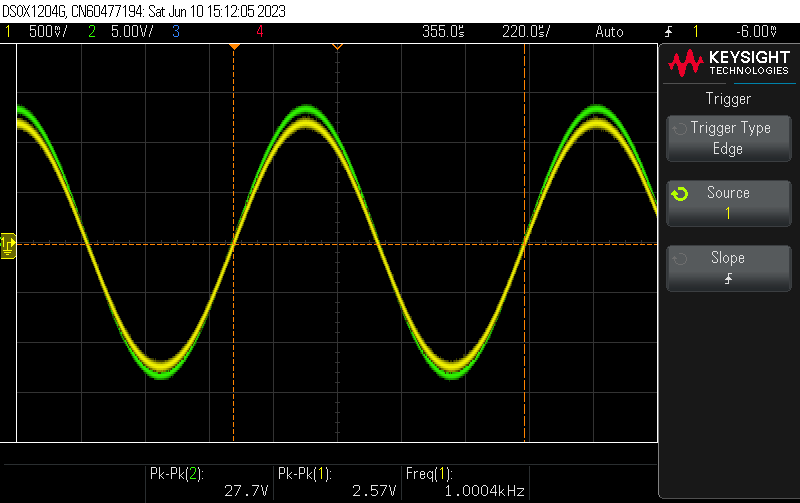
\includegraphics[height=7cm,width=10cm]{hihanten_2_4Vpp.png}
  \caption{FG出力が2.4Vppのときの非反転増幅回路のオシロスコープの波形}
\end{center}
\end{figure}
\begin{figure}[H]
  \begin{center}
  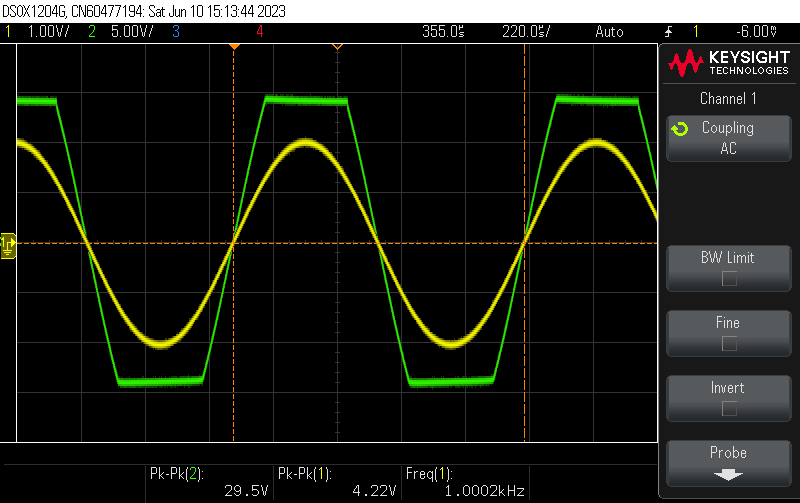
\includegraphics[height=7cm,width=10cm]{hihanten_4Vpp.png}
  \caption{FG出力が4.0Vppのときの非反転増幅回路のオシロスコープの波形}
\end{center}
\end{figure}
\begin{figure}[H]
  \begin{center}
  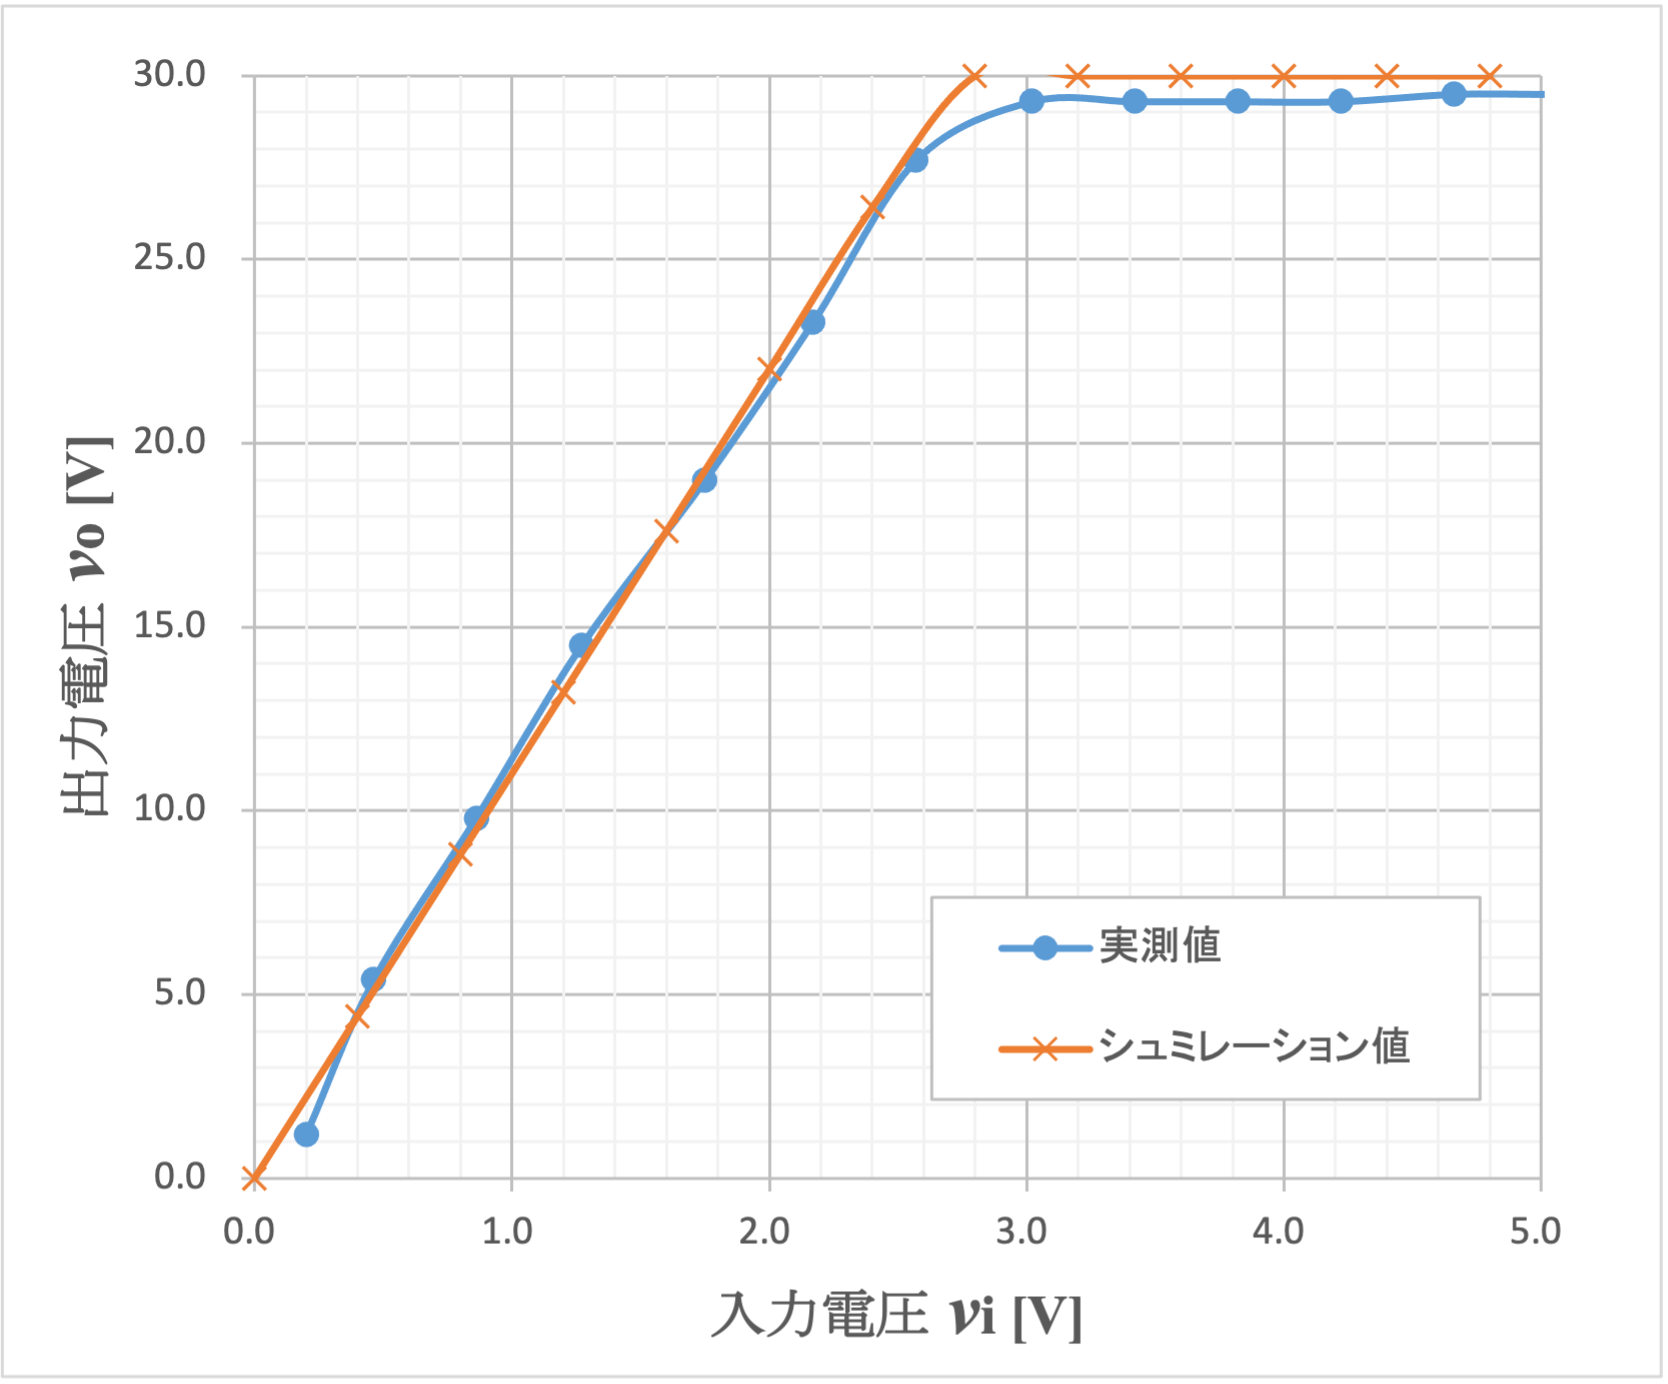
\includegraphics[height=7cm,width=10cm]{hihanpukugurafu.png}
  \caption{非反転増幅回路の電圧増幅特性}
\end{center}
\end{figure}
\subsection{加算回路}
まずそれぞれの抵抗を測定した値を示す.
$R_1$,$R_2$,$R_3$,$R_f$はそれぞれ9.97655$k\Omega$,9.96756$k\Omega$,9.98487$k\Omega$,9.9795$k\Omega$であった.
それぞれ測定したデータを示していく.
Δtは10$\mu$sを測定した後,0から40まで5$\mu$s刻みで測定した.波形は10,20,30$\mu$sのときの$v_2$測定時と$v_o$測定時のものを保存した.
\begin{figure}[H]
  \begin{center}
  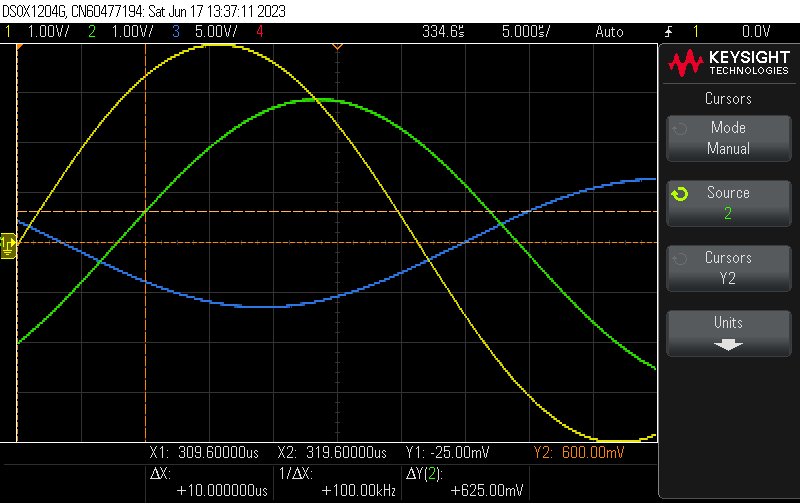
\includegraphics[height=7cm,width=10cm]{V2.png}
  \caption{$\Delta t$が10$\mu$sのときの$v_2$を測定したときの波形}
\end{center}
\end{figure}
\begin{figure}[H]
  \begin{center}
  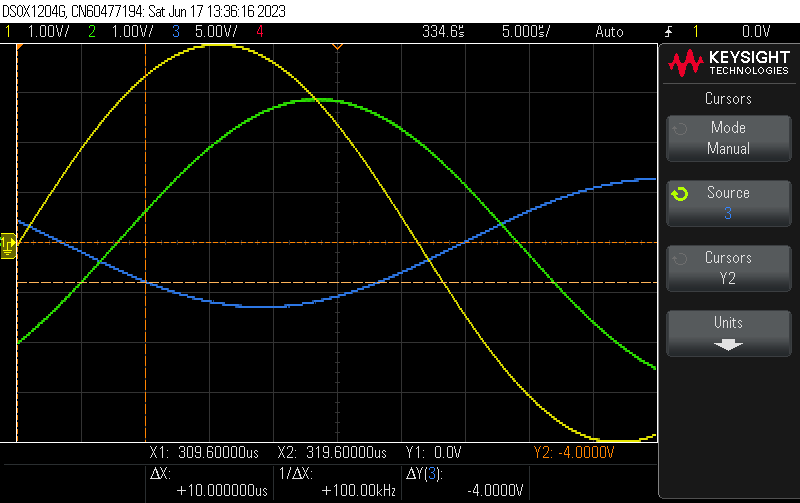
\includegraphics[height=7cm,width=10cm]{Vout.png}
  \caption{$\Delta t$が10$\mu$sのときの$v_o$を測定したときの波形}
\end{center}
\end{figure}
\begin{figure}[H]
  \begin{center}
  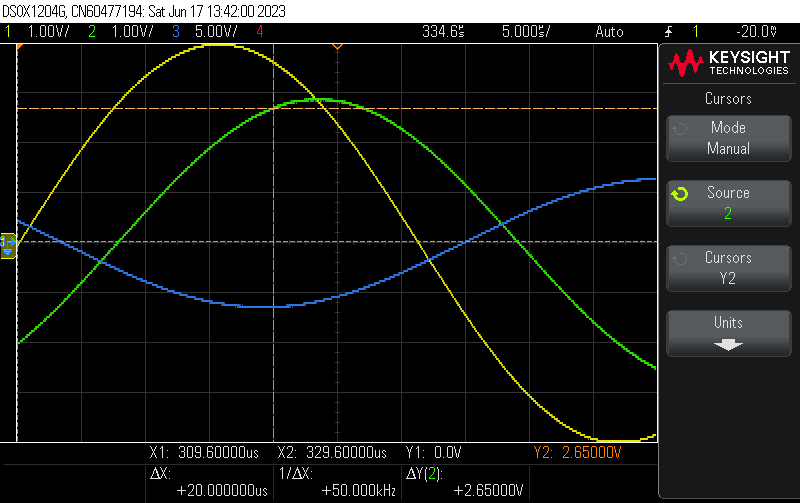
\includegraphics[height=7cm,width=10cm]{20_V2.png}
  \caption{$\Delta t$が20$\mu$sのときの$v_2$を測定したときの波形}
\end{center}
\end{figure}
\begin{figure}[H]
  \begin{center}
  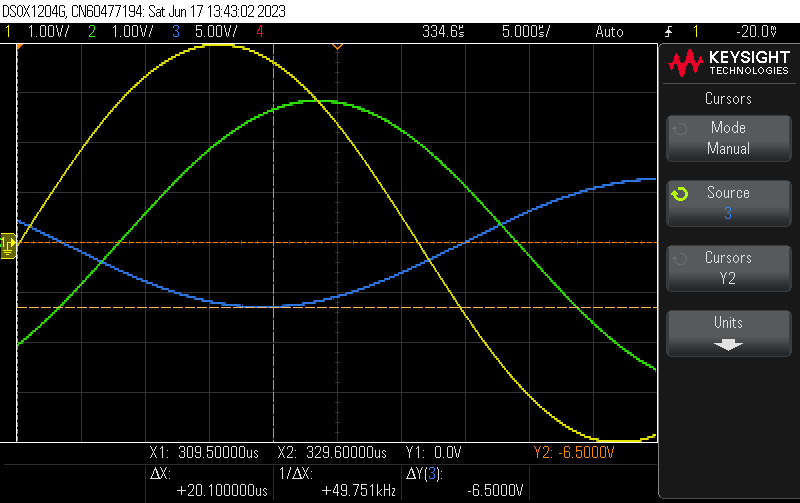
\includegraphics[height=7cm,width=10cm]{20_Vout.png}
  \caption{$\Delta t$が20$\mu$sのときの$v_o$を測定したときの波形}
\end{center}
\end{figure}
\begin{figure}[H]
  \begin{center}
  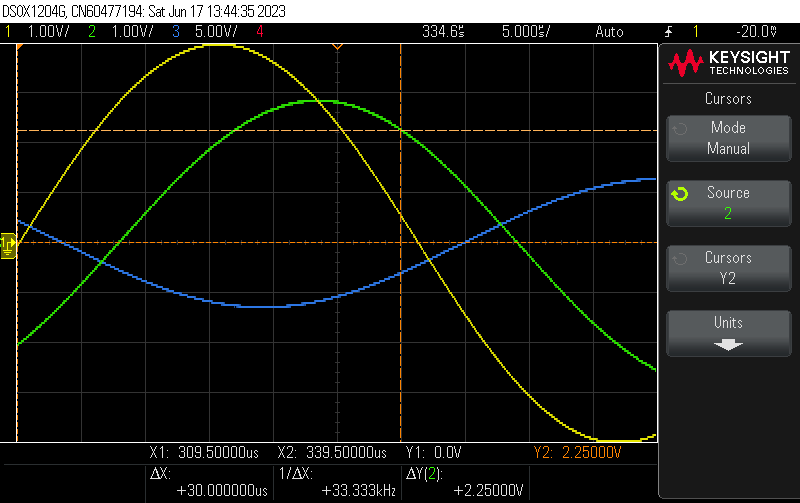
\includegraphics[height=7cm,width=10cm]{30_V2.png}
  \caption{$\Delta t$が30$\mu$sのときの$v_2$を測定したときの波形}
\end{center}
\end{figure}
\begin{figure}[H]
  \begin{center}
  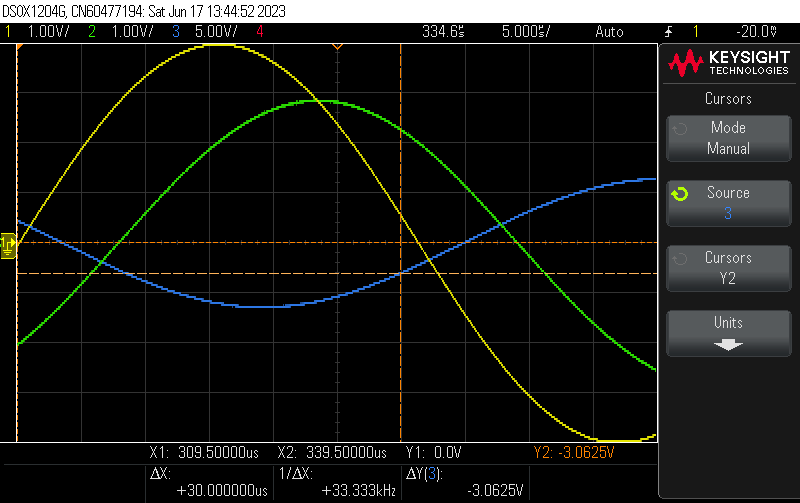
\includegraphics[height=7cm,width=10cm]{30_V2out.png}
  \caption{$\Delta t$が30$\mu$sのときの$v_o$を測定したときの波形}
\end{center}
\end{figure}

\begin{table}[H]
  \begin{center}
  \begin{tabular}{|l|l|l|l|l|}
  \hline
      Δt($\mu$s) & V1 & V2 & Vout & Vout計算値 \\ \hline
      0 & 0 & -1.95 & 1.95 & 1.952335878 \\ \hline
      5 & 1.8875 & -0.8 & -1.175 & -1.087099813 \\ \hline
      10 & 3.325 & 0.625 & -4 & -3.951731859 \\ \hline
      15 & 3.9 & 1.975 & -5.9 & -5.878519029 \\ \hline
      20 & 3.6 & 2.65 & -6.5 & -6.254238894 \\ \hline
      25 & 2.225 & 2.8 & -5.32 & -5.029011998 \\ \hline
      30 & 0.5 & 2.225 & -3 & -2.727813143 \\ \hline
      35 & -1.65 & 1 & 0.325 & 0.649290008 \\ \hline
      40 & -3.275 & -0.3875 & 3.5 & 3.663932577 \\ \hline
  \end{tabular}
  \caption{加算回路の測定結果}
\end{center}
\end{table}
この表をグラフにすると次のようになった.
\begin{figure}[H]
  \begin{center}
  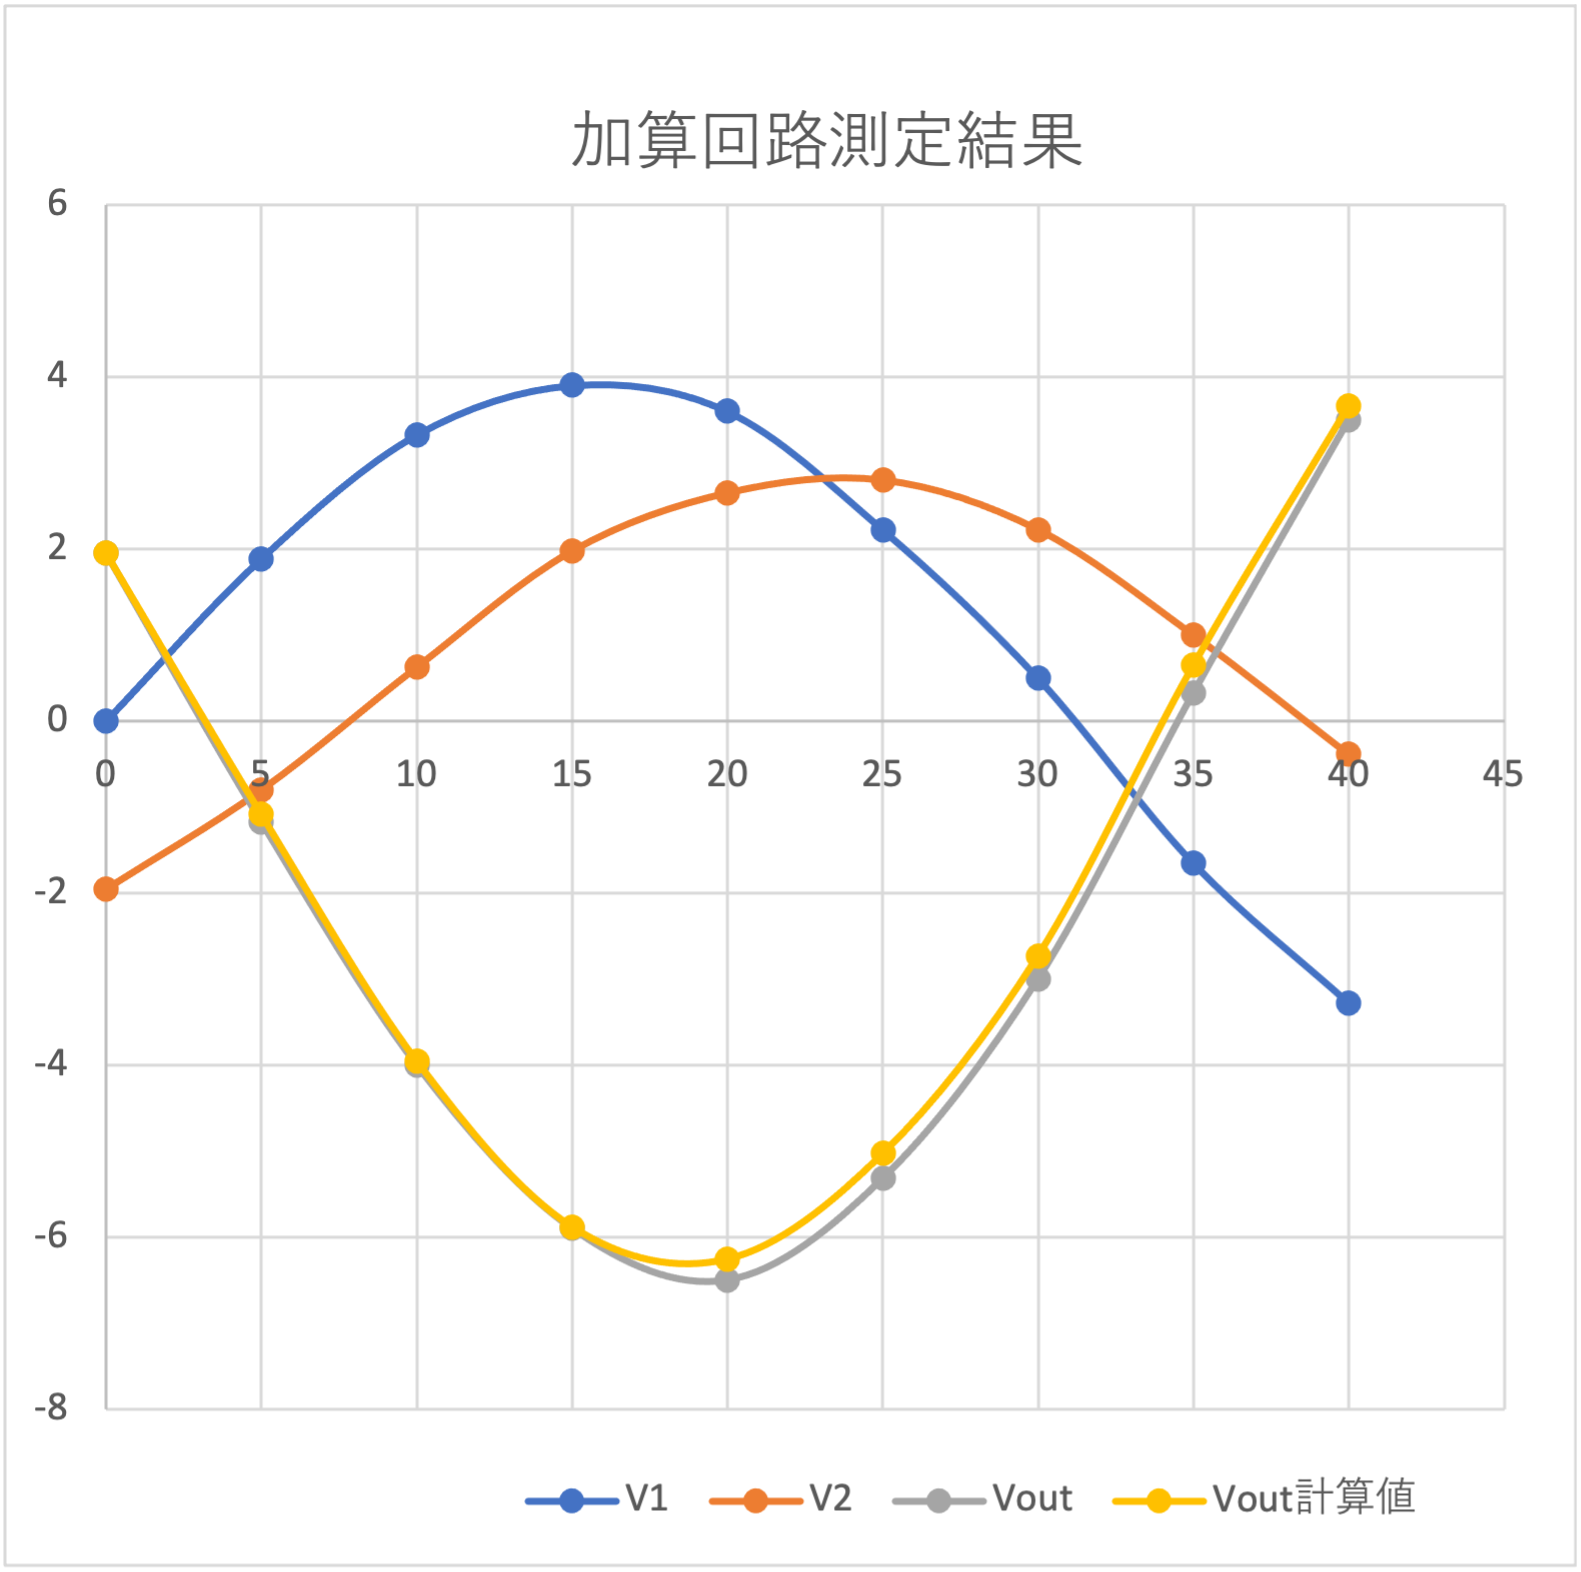
\includegraphics[height=7cm,width=10cm]{kasangurafu.png}
  \caption{加算回路の測定結果グラフ}
\end{center}
\end{figure}
\section{考察}
\subsection{1.反転増幅回路の理論値とシュミレーション値と実測値の比較}
反転増幅回路の増幅度の理論値は(\ref{Av})より-10.03倍となる.また増幅回路は出力が電源電圧以上になりえないのである一定の入力以上では増幅度が下がっていく.今回の実験では$V_o$は30V以上になり得ない.

シュミレーションでは1.2~1.4Vあたりをピークとして増幅度が下がっておりその最高値は-10.13倍,実測値では2.4Vppから増幅度が下がっており,最高値は-9.84倍となっている.
そうすると増幅度はシュミレーションと理論値では+0.1倍の差,実測値と理論値とでは-0.29倍の差がある.

非反転回路のほうでは理論値は
\begin{eqnarray}
  \label{A2}
A_V=1+\frac{R_2}{R_1}
\end{eqnarray}
となるので11.03倍となる.シュミレーションの最大の倍率は11.01倍,実測値の倍率は10.78倍となっており増幅度はシュミレーションと理論値では-0.2倍の差,実測値と理論値とでは-0.25倍の差がある.
\subsection{2.各回路の入力信号と出力信号の位相}
反転増幅回路は反転入力端子に信号を加えるため, 入力と出力の位相は反転する.これはシュミレーションの実験結果である図3を見て明らかである.
同様に図5,図6のオシロスコープの波形を確認しても位相が反転していることがわかる.

また非反転増幅回路は同位相となる結果がシュミレーションの図4となる.
同様に図8,図9のオシロスコープの波形を確認しても位相が反転していることがわかる.
\subsection{3.出力信号が頭打ちになる理由}
1.反転増幅回路の理論値とシュミレーション値と実測値の比較で触れた通り増幅回路では出力が電源電圧以上になりえないので,ある一定の入力以上では増幅度が下がっていく.
このことが確認できるのが図6,図9で$v_o$はある一定の値で増幅しなくなっている.
\subsection{4.加算回路の理論値と実測値の比較}
加算回路の$V_o$の値は(\ref{voqi})よりそれぞれ算出できる.
オシロスコープより$V_1$,$V_2$の値を計測し,$V_o$の理論値と実測値を確認する.
Δtが0$\mu$sのときは$V_1$は0なのであまり誤差がない.
それ以降の値を確認すると0.4Vより小さい程度理論値より大きくなっている.ほとんど理論値と同様の値になっている.これより適切に加算回路の測定が行われたと言える.
\subsection{5.応用例}
楽器等の音を増幅させるなどオーディオでの利用例が多い.
\section{まとめ}
反転増幅回路と加算回路の測定を通して,オペアンプの特性について学んだ.
オペアンプを利用した反転増幅回路,非反転増幅回路,加算回路の実装方法を理解し,そのほかにもウィーンブリッジ発振回路,コンパレータ回路の実装がオペアンプを用いてできることがわかった.

\begin{thebibliography}{9}
  \bibitem{a} 電気通信大学『アナログ回路実験』2023年,p23$\sim$30
 
\end{thebibliography}
\end{document}
